\chapter{ECS}
\label{chap:ecs}
V této kapitole si více rozebereme návrhový vzor ECS. Řekneme si, jak se implementuje ukládání komponent, rozebereme si vlastnosti ECS a na závěr porovnáme ECS s návrhovým vzorem Component.

\section{Reprezentace ECS}
To jak ECS funguje jsme si již zmínili v úvodu. Nyní si rozebereme jak bývají jednotlivé prvky ECS reprezentovány při jejich implementaci. Krom základních členů, jako jsou entity, komponenty a systémy, si představíme ještě world a query.

Komponenty, jako takové, bývají často reprezentovány třídou nebo strukturou. Jak již bylo zmíněno v úvodu, komponenty obsahují pouze data, nikoliv žádnou logiku. Proto tyto třídy a struktury neobsahují žádné funkce.

Entita by, podobně jako v návrhovém vzoru Component, mohla být reprezentována jako kolekce svých komponent. Ovšem to se v praxi nedělá, namísto toho se používá řešení, které vede k lepšímu výkonu. Konkrétně se dělá to, že každá ECS implementace má správce všech entit a komponent, ve kterém jsou jednotlivé komponenty uloženy. Jednotlivé entity jsou potom reprezentovány pouze jako jednoduchý identifikátor a je úlohou tohoto správce aby mapoval jednotlivé entity k jejich komponentám.

Tomuto správci se v ECS implementacích běžně říká world. Jak již bylo zmíněno, slouží jako správce a kontejner pro všechny entity a komponenty v herním světě. Jeho rozhraní nabízí funkce, pomocí niž je možné vytvářet a mazat jednotlivé entity. Často obsahuje také funkce pro přidávání a odebírání komponent jednotlivým entitám.

Některé ECS implementace reprezentují entity pomocí malé struktury, obsahující identifikátor dané entity společně s referencí na world do kterého patří. To umožňuje mít na této struktuře bohaté rozhraní s funkcemi pro přidávání a odebírání komponent.

Reprezentace systémů se v jednotlivých ECS implementacích dost liší. Některé vyžadují aby systém byl třída dědicí od abstraktního předka, jiné zase volí opačný extrém a dovolují systém reprezentovat téměř jakkoliv. Navzdory velkým odlišnostem se ve velkém počtu ECS implementací často objevuje objekt, který mohou používat jednotlivé systémy pro iterování entit s určitou množinou komponent.

Tomuto objektu se v ECS implementacích běžně říká query. Pro jeho vytvoření je většinou nutné poskytnou informaci, nad jakými typy komponent bude query pracovat. Je například možné mít query, které pracuje nad komponentami Movement a Position. Takové query by pak bylo schopné iterovat nad všemi entitami co mají komponenty Movement a Position. Pomocí tohoto query by bylo možné implementovat MovementSystem, který by řídil logiku pohybu.

% Query se dělí do dvou typů, statické a dynamické. Statické query je možné zkonstruovat (znamenaje také specifikovat typy komponent nad kterými bude pracovat) pouze za kompilace. Naproti tomu dynamické query je možné zkonstruovat za běhu. Dynamické query je poměrně pokročilá věc a pouze malé množství ECS implementací jej podporuje.

% Je důležité si uvědomit, že správa entit a komponent je dost složitá úloha. Je nutné aby bylo možné namapovat jednotlivé komponenty na jejich entity. Zároveň je také zapotřebí aby bylo možné iterovat určité n-tice těchto komponent za pomocí query. Je také důležité brát v potaz to, že jednotlivé entity a komponenty se mohou přidávat a odebírat za běhu. Více si o těchto věcech řekneme v pozdější sekci, nyní se ale zaměřme na mazání entit. Jelikož smazání takové entity může být naročné na implementaci a nebo také na výkon, některé ECS implementace využívajicí koncept tombstone. Tombstone je oznaceni pro objekt, ktery po smazani stale existuje, pouze je někde poznamenáno, že je již smazaný. Smazané entity bývají tedy v některých ECS implementacích označeny jako tombstone a query je při iteraci ignoruje.

%\section{Správa paměti}
%Než si rozeberem jak je možné úkládat komponenty, bude nutné si přiblížit jak vlastně funguje cache v počítači a také jaký je rozdíl mezi hodnotovími a referenčními typy v C\#.

%Cache

%Referencni vs hodnotove typy

\section{Ukládaní komponent}
Nyní si rozebereme způsoby, kterými jednotlivé ECS implementace řeší ukládání komponent v paměti. Většinou se rozlišují ECS implementace založené na \textit{sparse set} a ECS implementace založené na \textit{arch type}. Krom těchto dvou se poměrně často objevuje také třetí méně efektivní způsob ve kterém se jednotlivé komponenty ukládají pouze jako pointery, což má za následek špatný výkon.

\subsection{Arch type}
V ECS implementacích založených na \textit{arch type}, je \textit{arch type} typ entity. \textit{Arch type} je jednoznačně určen množinou komponent. Například mějme entitu představující postavu hráče, označme ji pro jednoduchost pouze jako entita hráče. Chceme aby náš hráč uměl chodit. Je nutné mu tedy přiřadit komponentu \verb|Position|, která reprezentuje jeho pozici v herním světě a také komponentu \verb|Movement|, která mu přidá schopnost pohybu. Jeho \textit{arch type}, označme ho \textit{arch type}~A, je tedy jednoznačně určen typy komponent \verb|Position| a \verb|Movement|. Jakákoliv jiná entita, která má pouze tyto dvě komponenty, také patří do \textit{arch type}~A. Dále mějme entitu stromu. Strom bude mít pouze komponentu \verb|Position|. Jeho \textit{arch type}, označme ho \textit{arch type}~B, je tedy jednoznačně určen typem komponenty \verb|Position|. Jakákoliv jiná entita, co bude mít také pouze komponentu \verb|Position| bude také patřit do \textit{arch type}~B.

Každá entity si uchovává odkaz na svůj \textit{arch type}. Jednotlivé \textit{arch type} jsou poté uloženy ve world. Každý \textit{arch type} v sobě obsahuje několik polí, konkrétně jedno pro každý typ komponenty. Každé entitě, je přiřazen identifikátor, který slouží jako index do těchto polí. Například \textit{arch type}~A má v sobě dvě pole, jedno pro \verb|Position| a jedno pro \verb|Movement|. Entita hráče má na sobě index~i, pomocí kterého je možné získat komponentu \verb|Position| nebo \verb|Movement|, která ji náleží. \textit{Arch type}~B má v sobě pouze jedno pole pro \verb|Position|. Entita stromu má na sobě index~j, pomocí kterého je možné získat komponentu \verb|Position|, která ji náleží.

Pokud poté vytvoříme query, které by mělo iterovat přes všechny entity s nějakou n-ticí komponent, tak toto query vezme vsechny \textit{arch type}, které obsahují danou n-tici a jednoduše projde příslušné pole. Například query, které by mělo iterovat přes entity s komponenty \verb|Position| a \verb|Movement|, vezme každý \textit{arch type} obsahující tyto dvě komponenty, v našem případě pouze \textit{arch type}~A, a projde příslušné pole. Pokud by query mělo iterovat přes entity s komponentou \verb|Position|, tak by prošlo pole pro \verb|Position| jak na \textit{arch type}~A tak na \textit{arch type}~B.

Velkou nevýhodou ECS implementacích založených na \textit{arch type} je přidávání a odebírání komponent. Pokud je některé entitě přidána nebo odebrána komponenta, dojde ke změně jejího \textit{arch type}. V takovém případě je nutné překopírovat všechny komponenty příslušné entity z původního \textit{arch type} do nového. Například pokud bychom entitě stromu přidali komponentu \verb|Resource|, která by reprezentovala suroviny, které hráč získá pokud jej pokácí, tak po přidání této komponenty by bylo nutné vzít \textit{arch type}, který je jednoznačně určen komponentami \verb|Position| a \verb|Resource|, a jednotlivé komponenty, v našem případě pouze \verb|Position|, do něj přesunout.

Přesouvání komponent může být výkonnostně náročná operace. Také je důležité si uvědomit, že přesouvání vyžaduje odebrání komponent z původního pole a to je O(n) operace. Ovšem tomuto se dá jednoduše předejít. Pokud nám nezáleží na pořadí prvků v poli, můžeme jednoduše vzít prvek, který chceme odebrat a prohodit ho s posledním prvkem v poli. Poté provedeme smazání posledního prvku. Tím dosáhneme smazání prvku z pole v čase O(1).

\subsection{Sparse set}

% \xxx{velikost packed nám dává kapacitu, velikost dense max prvek - upravit popis aby toto odrážel}
% - je potreba to odrazet?

\textit{Sparse set} je datová struktura, která reprezentuje množinu. Je možné do ní uložit čísla z množiny $0..u-1$. Na \textit{sparse set} je možné provádět operace vyhledání a vložení prvku v čase $O(1)$ a iteraci v čase $O(n)$. Rozbor této datové struktury je nad rámec této práce, proto pouze lehce nahlédneme na její implementaci.

\textit{Sparse set} se skládá ze dvou polí. Prvnímu se říká \textit{packed array} (někdy také \textit{internal array}, \textit{direct array}, nebo prostě \textit{values}). Druhé nese název \text{sparse array} (někdy také \textit{external array}, \textit{reverse array}, nebo prostě \textit{indices}). Obě tyto pole mají pevnou velikost. Pro \textit{packed array} je také stanovena kapacita, která odpovídá počtu prvků ve \textit{sparse set}. Příklad prázdného \textit{sparse set} pro $u=6$ je možné vidět na obrázku \ref{fig:sparse_set_empty}. 

\begin{figure}
    \centering
    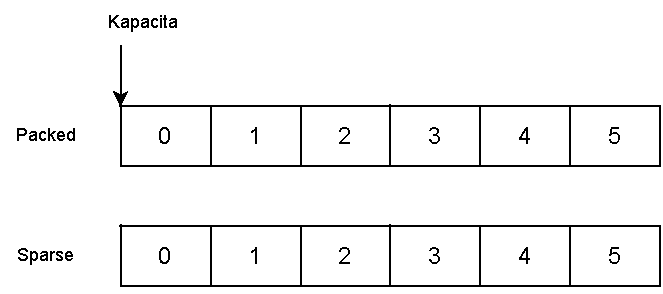
\includegraphics[width=0.6\linewidth]{img/sparse_set_empty.pdf}
    \caption{Příklad prázného sparse set pro u=6.}
    \label{fig:sparse_set_empty}
\end{figure}

Při jakékoliv operace platí pro \textit{sparse set} následující invariant: $\forall v \in \text{sparse}: \text{packed}\left[\text{sparse}\left[v\right]\right] = v$. Jak je vidět na obrázku \ref{fig:sparse_set_empty}, tento invariant platí také pro prvky, které nejsou součástí \textit{sparse set}.

Nahlédněme prvně na operaci přidání prvku. Pokud bychom chtěli přidat prvek který se nachází hned za hranicí naší kapacity, konkrétně prvek $\text{packed}\left[\text{kapacita}\right]$ (v případě obrázku \ref{fig:sparse_set_empty} se jedná o prvek $0$), stačí nám zvýšit kapacitu o $1$. Tuto situaci můžeme vidět na obrázku \ref{fig:sparse_set_one}. V případě, že chceme přidat prvek, který se nachází na pozici $i$, kde $i > \text{kapacita}$, je nutné nejprve prohodit prvky $\text{packed}\left[\text{kapacita}\right]$ a $\text{packed}\left[i\right]$. Aby nedošlo k porušení invariantu, je také nutné prohodit odpovídající prvky v \textit{sparse array}. Po prohození prvků můžeme postupovat stejně jako v prvním případě. Tuto situaci můžeme vidět na obrázku \ref{fig:sparse_set_two}.

\begin{figure}
    \centering
    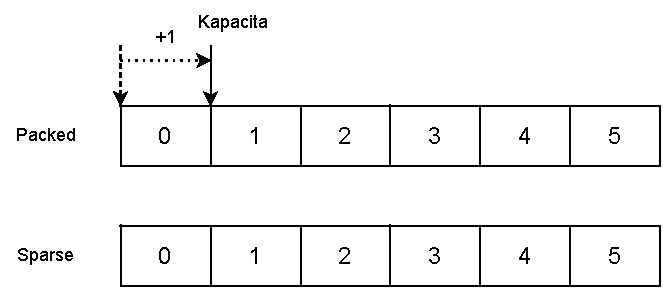
\includegraphics[width=0.6\linewidth]{img/sparse_set_one.pdf}
    \caption{Příklad našho sparse set po přidání prvku, který se nachází hned za hranicí kapacity.}
    \label{fig:sparse_set_one}
\end{figure}

\begin{figure}
    \centering
    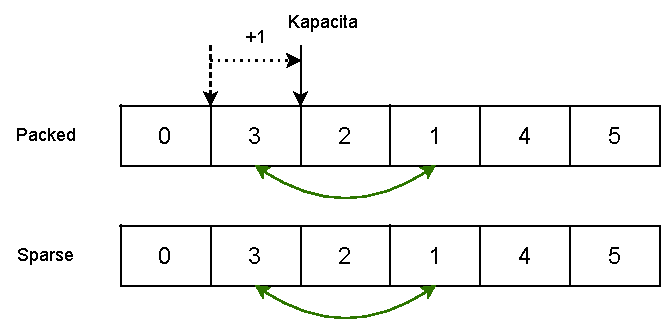
\includegraphics[width=0.6\linewidth]{img/sparse_set_two.pdf}
    \caption{Příklad našeho sparse set po přidání obecného prvku. Nejprve je nutné prohodit prvek, který chceme přidat s prvkem za hranicí kapacity, poté dojde k navýšení kapacity.}
    \label{fig:sparse_set_two}
\end{figure}

Přidejme si do našeho pole další dva prvky, konkrétně $2$ a $1$. Přidání provedeme v tomto pořadí. Současnou situaci je možné vidět na obrázku \ref{fig:sparse_set_four}. Nyní bychom chtěli nějaký prvek odebrat. V jednoduchém případě, kdy je náš prvek těsně před hranicí kapacity, konkrétně se jedná o prvek $\text{packed}\left[\text{kapacita - 1}\right]$ (v případě obrázku \ref{fig:sparse_set_four} prvek 1), stačí nám zmenšit kapacitu o $1$. Pokud se jedná o jiný prvek, tak podobně jako při odebírání, prohodíme tento prvek s prvkem $\text{packed}\left[\text{kapacita - 1}\right]$. Obdobně jako u odebíraní je nutné prohodit odpovídající prvky v \textit{sparse array} aby nedošlo k porušení invariantu. Poté postupujeme jako v prvním případě. Příklad druhé situace můžeme vidět na obrázku \xxx{sparse\_set\_three}.

\begin{figure}
    \centering
    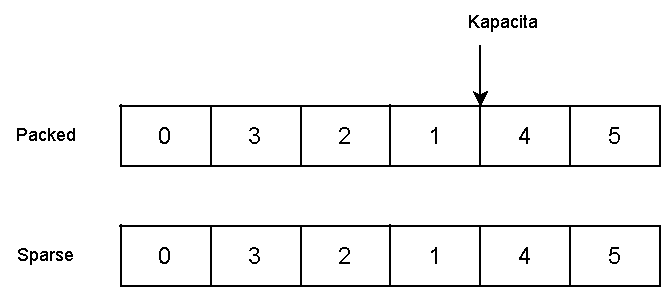
\includegraphics[width=0.6\linewidth]{img/sparse_set_four.pdf}
    \caption{Příklad našeho sparse set po přidání prvků 2 a 1.}
    \label{fig:sparse_set_four}
\end{figure}

\begin{figure}
    \centering
    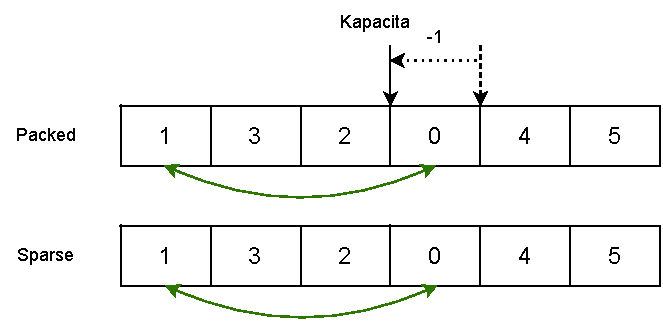
\includegraphics[width=0.6\linewidth]{img/sparse_set_three.pdf}
    \caption{Příklad našeho sparse set po odebraní obecného prvku. Nejprve je nutné prohodit prvek, který chceme odebrat s prvek před hranicí kapacity, poté dojde ke snížení kapacity.}
    \label{fig:sparse_set_three}
\end{figure}

\xxx{Jak se používá sparse set v ECS.}

\subsection{Jiné způsoby ukládání komponent}
Komponenty jako pointery

\section{Vlastnosti ECS}
...

Vysoka flexibilita

Vysoky vykon

Flexibilita > vykon

\section{ECS vs Component}

\xxx{TODO}

\xxx{maybe topics: dynamicke vs staticke query, tombstones, relace, eventy, tag component, system types, reaction systems, paralelism, paralel queries, query filters, functional programming, relace, eventy, prukopnici (herni engine Bevy, ECS knihovny entitas a flecs)}